\documentclass[]{report}
\usepackage{listings}
\usepackage{tikz}
\usetikzlibrary{shapes.geometric, arrows}

%tikx styles
\tikzstyle{startstop} = [rectangle, rounded corners, minimum width=2.5cm, minimum height=0.6cm,text centered, draw=black, fill=red!30, align=center]
\tikzstyle{io} = [trapezium, trapezium left angle=70, trapezium right angle=110, minimum width=2.5cm, minimum height=0.6cm, text centered, draw=black, fill=blue!30, align=center]
\tikzstyle{process} = [rectangle, minimum width=2.5cm, minimum height=0.6cm, text centered, draw=black, fill=orange!30, align=center]
\tikzstyle{decision} = [diamond, minimum width=2.5cm, minimum height=0.6cm, aspect=2, text centered, draw=black, fill=green!30, align=center]
\tikzstyle{arrow} = [thick,->,>=stealth]

% Title Page
\title{Using the Submitter class for high throughput HPC calculations with Soprano}
\author{Simone Sturniolo}

\begin{document}
\maketitle

\chapter{The Submitter class}

In Soprano, the \lstinline|hpc.submitter| module provides classes and tools meant to help computational scientists to automate the process of generating, running and possibly post-processing huge batches of molecular calculations like molecular dynamics, DFT calculations and so on on high performance computing machines where access to the nodes is regulated by a queueing system. The target is to allow users to create their own pipelines for high throughput calculations, like running the same analysis tools through an entire database of chemical structures, with only a few lines of Python code. Since this is, however, still a complex task that will inevitably require to be customised and tailored to the needs of each specific case, using this functionality requires a somewhat higher level of programming confidence than the rest of the library and can look a little daunting at first. No worries - this manual will guide you through the steps necessary to deploy your own Submitter to your machine of interest to run potentially any computational task you can think of. Besides instructions on the creation of a new Submitter, this manual also will include advice on how to test it and debug it locally, in order to minimise the risk of running into bugs after deploying the system.\newline
First, let us clarify what a Soprano Submitter instance \textit{is} and \textit{isn't}. A Submitter is a very general class designed to automate the process of queueing, running and postprocessing huge amounts of calculations on a computing cluster. It is \textit{not}:
\begin{itemize}
	\item a system designed to push calculations to a remote machine. A Soprano Submitter is meant to be run on the same machine where the calculations are going to be run;
	\item a system handling parallel calculations. There is no parallelism included in a Submitter. As the name suggests, it simply submits jobs to a queueing system like GridEngine, which then itself provides them with the required number of cores. The Submitter is entirely agnostic of the underlying hardware architecture; 
	\item a system ready for deployment as-is. As it comes shipped with Soprano, the Submitter class basically does nothing. It is meant to be used as a parent class to write your own sub-class which specifies the details of the task of interest through a number of designated methods. This is absolutely on purpose - the objective here is maximum flexibility for potentially very demanding tasks, sacrificing immediate usability.
\end{itemize}

Now let's see a quick overview of what the typical pipeline for deploying a Submitter system is, followed by a more detailed explanation of all the steps involved.

\chapter{Deploying a Submitter}

The process to create and launch a Submitter requires the following steps:

\begin{itemize}
	\item Write a class inheriting from \lstinline|soprano.hpc.submitter.Submitter| implementing the desired calculation through its core methods;
	\item Write a Python source file creating an instance of this class (it can also be the same file) and setting up its parameters, and positioning this file in the working directory. In some cases this might require creating a \lstinline|soprano.hpc.submitter.QueueInterface| as well;
	\item Create a submission script for your HPC system using tags which are going to be replaced by specific values in each job;
	\item Launch the newly created submitter from the command line by calling the appropriate Soprano script.
\end{itemize}

Let's see these steps in more detail.

\section{Writing a Submitter class}

The basic template to inherit from the Submitter class can be as simple as this:

\begin{lstlisting}
from soprano.hpc.submitter import Submitter

class MySubmitter(Submitter):
	pass
\end{lstlisting}

However, such a class would be of no use since it does not implement any particular behaviour. The Submitter class originally has a number of methods. Some of them are preceded by an underscore and are meant to not be touched, as they handle the core behaviour of any Submitter. Others are meant to be overridden when inheriting from the base class and control custom behaviour - the specifics of the problem at hand. The core methods determine the Submitter workflow, which can be described as follows:

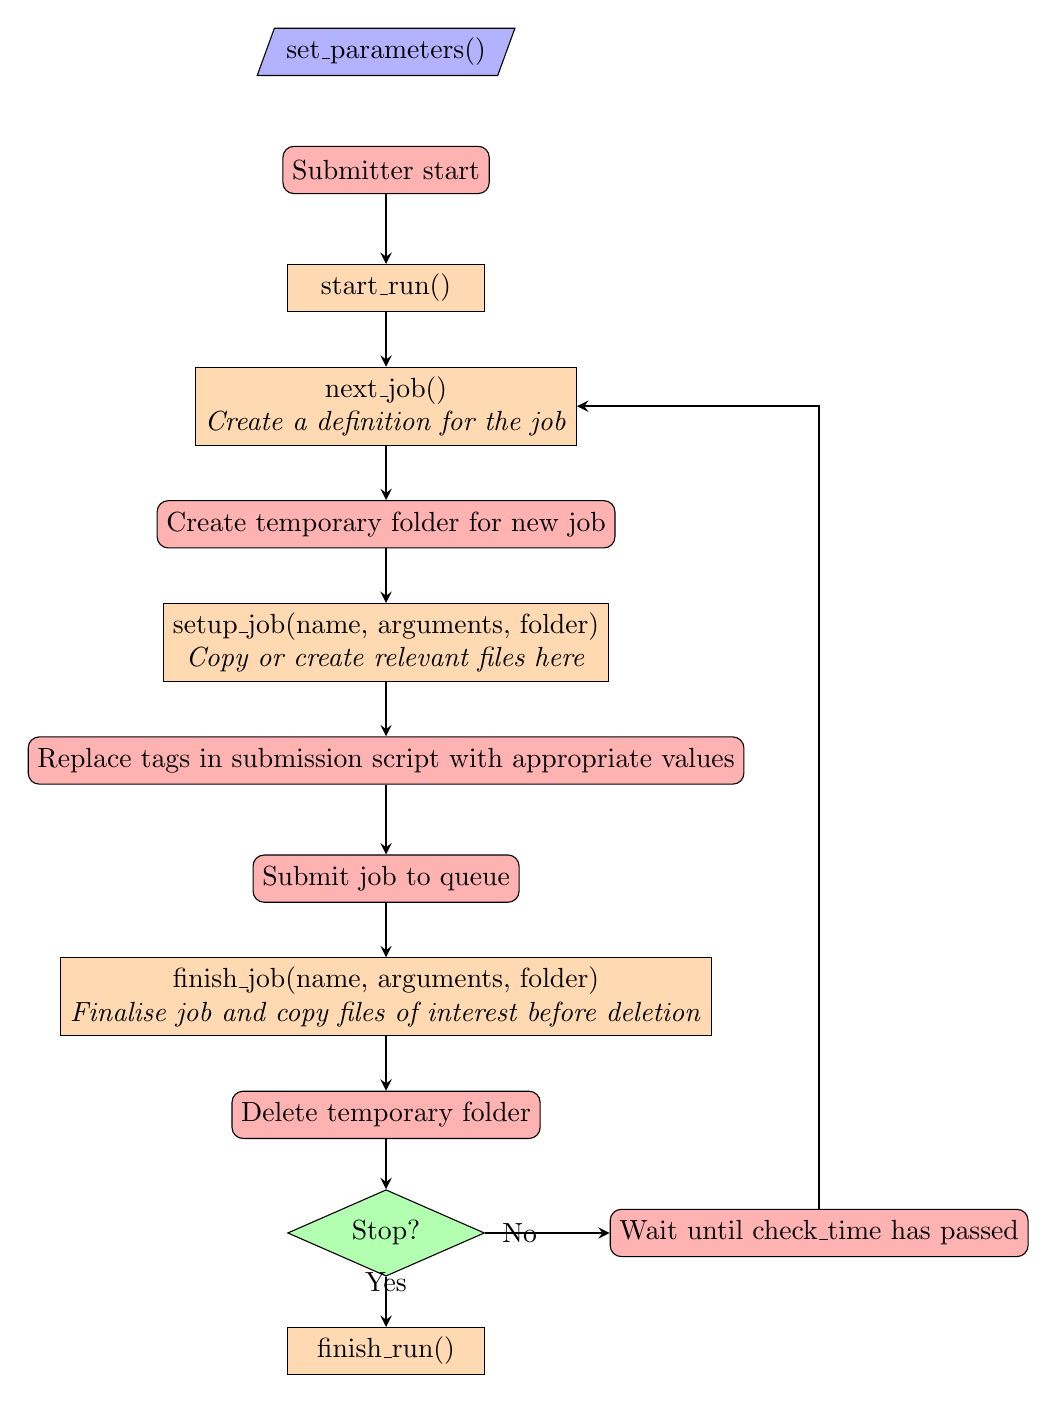
\begin{tikzpicture}[node distance=1.5cm]

\node (in1) [io] {set\_parameters()};
\node (start) [startstop, below of=in1] {Submitter start};
\node (startrun) [process, below of=start] {start\_run()};
\node (nextjob) [process, below of=startrun] {next\_job()\\\textit{Create a definition for the job}};
\node (makedir) [startstop, below of=nextjob] {Create temporary folder for new job};
\node (setupjob) [process, below of=makedir] {setup\_job(name, arguments, folder)\\\textit{Copy or create relevant files here}};
\node (tagscript) [startstop, below of=setupjob] {Replace tags in submission script with appropriate values};
\node (runjob) [startstop, below of=tagscript] {Submit job to queue};
\node (finjob) [process, below of=runjob] {finish\_job(name, arguments, folder)\\\textit{Finalise job and copy files of interest before deletion}};
\node (deldir) [startstop, below of=finjob] {Delete temporary folder};
\node (finished) [decision, below of=deldir] {Stop?};
\node (continue) [startstop, right of=finished, xshift=4cm] {Wait until check\_time has passed};
\node (finishrun) [process, below of=finished] {finish\_run()};

\draw [arrow] (start) -- (startrun);
\draw [arrow] (startrun) -- (nextjob);
\draw [arrow] (nextjob) -- (makedir);
\draw [arrow] (makedir) -- (setupjob);
\draw [arrow] (setupjob) -- (tagscript);
\draw [arrow] (tagscript) -- (runjob);
\draw [arrow] (runjob) -- (finjob);
\draw [arrow] (finjob) -- (deldir);
\draw [arrow] (deldir) -- (finished);
\draw [arrow] (finished) -- node[anchor=east] {No} (continue);
\draw [arrow] (continue) |- (nextjob);
\draw [arrow] (finished) -- node[anchor=south] {Yes} (finishrun);

\end{tikzpicture}



\end{document}          
